% !TEX program = xelatex
% 光遗传学视觉恢复 · 论文取材命题（上海生物等级考风格）
% 编译：xelatex -interaction=nonstopmode -halt-on-error 本文件（跑两遍）
\documentclass[UTF8,a4paper,11pt]{ctexart}

\usepackage{geometry}
\geometry{left=1.9cm,right=1.9cm,top=2.3cm,bottom=2.3cm}
\usepackage{graphicx}
\usepackage{amsmath,amssymb}
\usepackage{booktabs}
\usepackage{longtable}
\usepackage{array}
\usepackage{enumitem}
\usepackage{xcolor}
\usepackage{caption}
\usepackage{float}
\usepackage{titlesec}
\usepackage{fancyhdr}
\usepackage[hidelinks]{hyperref}

\graphicspath{{../命题图/}{../../Resources/Downloads/原图-光遗传学视觉恢复/}}

\definecolor{deepblue}{HTML}{1F4E79}
\definecolor{deepred}{HTML}{C00000}
\definecolor{deepgreen}{HTML}{2E7D32}

\captionsetup{font=small,labelfont=bf}
\titleformat{\section}{\Large\bfseries\color{deepblue}}{\thesection}{0.6em}{}
\titleformat{\subsection}{\large\bfseries\color{deepblue}}{\thesubsection}{0.6em}{}
\pagestyle{fancy}
\fancyhf{}
\fancyhead[L]{\small 光遗传学视觉恢复 · 论文取材命题（上海风格）}
\fancyhead[R]{\small\thepage}

\newcommand{\ans}{\par\medskip\noindent\textbf{\color{deepblue}【参考答案与解析】}\par\smallskip}
\newcommand{\pt}[1]{\textbf{（#1分）}}
\newcommand{\key}[1]{\textbf{\color{deepred}#1}}
\newcommand{\tian}[1]{\underline{\hspace{#1}}}
% 题型标签
\newcommand{\tg}[1]{{\small\color{deepgreen}［#1］}}
\newcommand{\choice}[1]{\par\smallskip\noindent #1\par}

\title{\bfseries 光遗传学视觉恢复\\[4pt]\large 论文取材命题（上海生物等级考风格 · 题型对齐版）\\[6pt]
\normalsize 取材：Pan 实验室三篇开放获取论文；配图以论文原图为主}
\author{}
\date{2026-10-06}

\begin{document}
\maketitle
\thispagestyle{fancy}

\begin{center}
\fbox{\parbox{0.95\textwidth}{\small
\textbf{短标题待定}（候选：\emph{送光入眼}／\emph{复明的开关}／\emph{给盲鼠一束光}／\emph{光控复明}）。\\
本题组共 4 道大题、22 个小题，合计 44 分；其中\textbf{单选、多选、编号选填、编号排序四类客观题共 14 题（约 64\%）}，
与上海卷"题型稳定，包括单选、多选、编号选填、填空、简答等"的分布一致。\textbf{推荐优先使用：题一}。
}}
\end{center}

\section*{命题说明}
\addcontentsline{toc}{section}{命题说明}

\subsection*{一、上海卷出题风格分析（依据官方点评）}

上海市教育考试院历年对等级考生物卷的官方点评，给出了可操作的命题特征：

\begin{longtable}{@{}p{3.4cm}p{11.4cm}@{}}
\toprule
\textbf{风格特征} & \textbf{官方表述与本卷落实方式} \\
\midrule
\endhead
情境化组卷 & "试卷中\textbf{六大问题皆出自真实情境}""六道大题均以真实科研或社会问题为情境"——本卷每道大题对应一个真实课题（三篇原始论文），不以知识点堆砌成题。 \\
题型稳定 & "试卷题型稳定，包括\textbf{单选、多选、编号选填、填空、简答}等"——本卷四类客观题共 14 题，占比约 64\%。 \\
设问递进 & "试题的设置\textbf{由浅入深、层层递进}，从核心概念的理解到具体问题的分析，再到复杂机制的推理或解决方案的提出"——每道大题内部按 识记→图表分析→机制推理→方案设计 排列。 \\
宏微结合 & "让学生从\textbf{图表的信息中提炼、区分、归纳}出细胞接受与传递信息的特点"——本卷大量使用论文原图作为信息载体。 \\
工程与探究 & "考查学生是否能\textbf{用基因工程的基本原理}……设计合理的实践方案，实现工程目标""提出合理的\textbf{实验方案}"——题一、题三分别对准工程方案与实验设计。 \\
\bottomrule
\end{longtable}

\noindent\textbf{客观题评分约定}（本卷统一采用，可按需调整）：单选每题 2 分；多选每题 2 分，\textbf{选对但不全得 1 分，错选得 0 分}；编号选填每题 2 分，同多选规则；编号排序每题 2 分，\textbf{顺序完全正确得 2 分，错一处得 1 分，错两处及以上得 0 分}。

\subsection*{二、取材论文与配图}

\begin{longtable}{@{}p{0.4cm}p{5.6cm}p{2.4cm}p{6.0cm}@{}}
\toprule
\textbf{\#} & \textbf{文献} & \textbf{期刊/年} & \textbf{本卷使用的原图} \\
\midrule
\endhead
1 & Lu Q, Ganjawala TH, Ivanova E, Cheng JG, Troilo D, \textbf{Pan ZH}. AAV-mediated transduction and targeting of retinal bipolar cells with improved mGluR6 promoters in rodents and primates & \textit{Gene Therapy}, 2016 & Fig.~1（mGluR6 序列与调控元件示意）／Fig.~4（mCherry 与 PKC 共标）／Fig.~8（灵长类视网膜） \\
2 & Lu Q, Ganjawala TH, Hattar S, Abrams GW, \textbf{Pan ZH}. A robust optomotor assay for assessing the efficacy of optogenetic tools for vision restoration & \textit{IOVS}, 2018 & Fig.~1（自制视动装置）／Fig.~3（瞳孔对光收缩比较）／Fig.~4（OMR 阈值光强—空间频率）／Fig.~5（阿托品阻断瞳孔收缩） \\
3 & \textbf{Pan ZH}, Ganjawala TH, Lu Q, Ivanova E, Zhang Z. ChR2 mutants at L132 and T159 with improved operational light sensitivity for vision restoration & \textit{PLoS ONE}, 2014 & 见附录 A（用于"定点突变"设问） \\
\bottomrule
\end{longtable}

\noindent 全部 22 张原图与两篇全文（Markdown）、一篇原版 PDF 已入库 \texttt{00 - Personal/Resources/Downloads/}。本卷\textbf{以论文原图为主要配图}；重绘图（图P1、图P2）仅在原图缺少"视网膜三级通路与病变位置""基因盒与调控元件"这类示意时补充使用，并集中于附录 B 对照。

\subsection*{三、题型分布}

\begin{table}[H]
\centering\small
\begin{tabular}{@{}lccccccc@{}}
\toprule
\textbf{大题} & \textbf{单选} & \textbf{多选} & \textbf{编号选填} & \textbf{编号排序} & \textbf{填空} & \textbf{简答/设计} & \textbf{分值} \\
\midrule
题一（★推荐·综合取材） & 1 & 1 & 1 & 1 & 1 & 1 & 12 \\
题二（结构与功能/图表） & 1 & 1 & 1 & 1 & 1 & 0 & 10 \\
题三（实验设计） & 1 & 1 & 0 & 1 & 0 & 2 & 12 \\
题四（跨学科定量） & 1 & 1 & 1 & 0 & 1 & 1 & 10 \\
\midrule
\textbf{合计} & \textbf{4} & \textbf{4} & \textbf{3} & \textbf{3} & \textbf{3} & \textbf{4} & \textbf{44} \\
\bottomrule
\end{tabular}
\end{table}

\clearpage
\section{题一（★推荐）· 论文取材综合题}
\addcontentsline{toc}{section}{题一（★推荐）· 论文取材综合题}

\subsection*{材料}

视网膜色素变性（RP）是一类由基因突变引起的遗传性眼病：患者视网膜中的\textbf{感光细胞}逐渐死亡，而其内层的\textbf{双极细胞}与\textbf{神经节细胞}大多仍然存活（图P1）。因此，仅仅修复致病基因并不能恢复患者的视力。

研究者的思路是：把一种来自单细胞藻类的光敏蛋白——\textbf{通道视紫红质（ChR2）}的基因，用\textbf{腺相关病毒（AAV）}作载体送入视网膜。要让这一基因只在特定细胞里"定点开灯"，必须在基因前连接合适的\textbf{调控元件}（图T1）。2014 年，研究者还在 ChR2 的 132 位和 159 位氨基酸对应位点上构建了多种\textbf{突变体}，以提高弱光下的反应能力；2018 年，他们把这些变体分别导入\textbf{三敲除失明小鼠}（视杆细胞、视锥细胞与黑视素均缺失）的视网膜内层神经元，用"视动反应（OMR）"与"瞳孔对光收缩"评价视功能恢复情况（结果见题三）。

\begin{figure}[H]
\centering
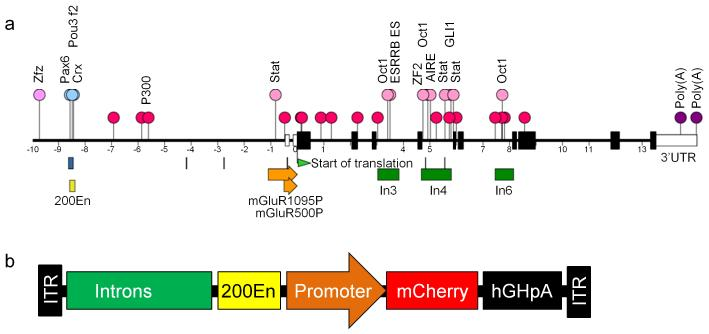
\includegraphics[width=1.0\textwidth]{Lu2016-Fig01.jpg}
\caption{图T1\quad 论文原图（Lu et al., \textit{Gene Therapy}, 2016, Fig.~1）：mGluR6 基因及其上下游序列示意，白框为用于驱动目的基因表达的候选序列。}
\end{figure}

\begin{figure}[H]
\centering
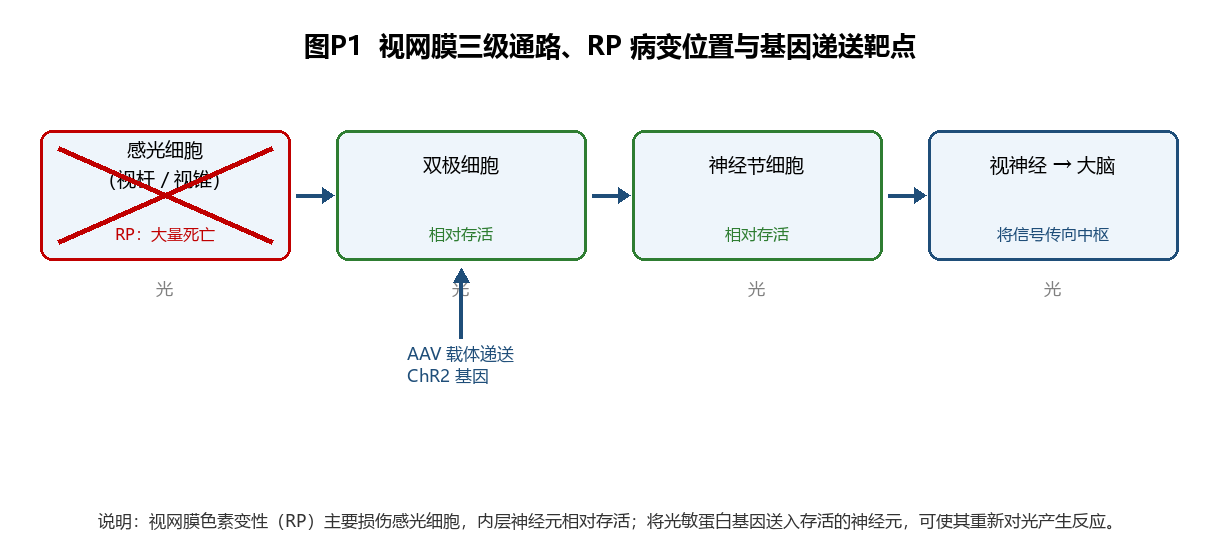
\includegraphics[width=0.92\textwidth]{P1_视网膜三级通路与病变.png}
\caption{图P1\quad 视网膜三级通路、RP 病变位置与基因递送靶点（重绘，用于补足原图未涉及的通路示意）}
\end{figure}

\subsection*{设问（共 12 分）}

\begin{enumerate}[leftmargin=2.1em,itemsep=5pt]
\item \tg{单选} \pt{2} 在\textbf{未导入光敏蛋白的正常}视网膜中，能把光信号转变为电信号的细胞是（\quad）\\
\choice{A. 双极细胞 \quad B. 感光细胞（视杆与视锥） \quad C. 神经节细胞 \quad D. 水平细胞}

\item \tg{多选} \pt{2} 关于"把 ChR2 表达在视网膜内层神经元以恢复视觉"，下列叙述正确的有（\quad）（错选得 0 分）\\
\choice{A. RP 中感光细胞大量死亡，而双极细胞大多存活\\
B. ChR2 使表达它的细胞在蓝光照射下发生离子流动，从而产生电位变化\\
C. 实现该过程需要向细胞内导入外源基因\\
D. 细胞表达 ChR2 后，视觉信号可不再经过神经节细胞}

\item \tg{编号选填} \pt{2} 图T1 中，标注为白色方框的序列位于翻译起点\textbf{上游}、且被连接在目的基因前用于驱动其表达。它们最可能属于（\quad）（填编号）\\
\choice{① 编码区 \quad ② 调控元件（启动子、增强子） \quad ③ 内含子 \quad ④ 终止子}

\item \tg{编号排序} \pt{2} 用编号和箭头（→）表示"使视网膜双极细胞对蓝光产生反应"的主要过程顺序：\\
\choice{① 目的基因转录并翻译出 ChR2 蛋白 \quad ② 构建含 ChR2 基因的重组载体\\
③ 载体进入视网膜细胞 \quad ④ ChR2 定位到细胞膜上，形成光控离子通道\\
答：\tian{6.2cm}}

\item \tg{填空+简答} \pt{2} 2014 年研究者对 ChR2 基因进行定点突变以提高光敏性。该变异属于\tian{2.6cm}（填"基因重组""基因突变"或"染色体变异"）；\\
从"\textbf{基因突变 → 蛋白质结构 → 功能}"的角度，说明这种改造为什么能提高细胞对弱光的敏感度：\tian{0.5\textwidth}

\item \tg{简答} \pt{2} 研究者在啮齿类之后又在\textbf{灵长类}视网膜上重复了实验。请说明这样做的意义，并写出该技术走向临床应用仍面临的一个限制。\tian{0.5\textwidth}
\end{enumerate}

\ans
\begin{enumerate}[leftmargin=2.1em,itemsep=3pt]
\item \textbf{B}。感光细胞（视杆、视锥）是视网膜中感受光刺激并把光信号转变为电信号的细胞；双极细胞与神经节细胞是其后逐级传递信号的神经元。
\item \textbf{ABC}。A、B、C 正确；\textbf{D 错}——神经节细胞是视网膜的输出神经元，其轴突构成视神经，信号必须经它上传至中枢，表达 ChR2 只是\textbf{绕过死亡的感光细胞}，并未绕过神经节细胞。
\item \textbf{②}。白色方框位于翻译起点上游且为\textbf{非编码序列}，其作用是调控下游基因"在哪里、表达多少"，属于启动子／增强子这类调控元件。
\item \textbf{②→③→①→④}。先构建重组载体（②），导入细胞（③），基因转录翻译出 ChR2（①），蛋白定位到膜上形成通道（④）。
\item \textbf{基因突变}；\textbf{原理}：定点突变改变了 ChR2 基因的\textbf{碱基（对）序列}，使蛋白质中相应位置的\textbf{氨基酸被替换}，进而改变蛋白质的\textbf{空间结构}，使该离子通道在光照下更易开放（弱光下光电流更大），细胞对弱光的敏感度因而提高。
\item \textbf{意义}：灵长类的眼球结构与视网膜细胞组成比啮齿类\textbf{更接近人}，在灵长类上验证可检验该策略的可行性与安全性，为临床转化提供更可靠的依据。\\
\textbf{限制}（答出一点即可）：① 需向人体导入外源基因，存在免疫反应、插入突变等安全性与伦理问题；② 光在眼内的穿透与投递受瞳孔、屈光介质限制；③ 目前恢复的只是光感／运动检测，与正常视觉差距很大；④ 载体长期表达的稳定性与剂量控制尚待解决。
\end{enumerate}

\clearpage
\section{题二 · 结构与功能／图表分析型}
\addcontentsline{toc}{section}{题二 · 结构与功能／图表分析型}

\subsection*{材料}

视网膜色素变性（RP）患者的\textbf{感光细胞}逐渐死亡，而内层神经元大多存活。为让存活的内层神经元重新对光敏感，研究者把携带 ChR2 基因的 AAV 载体注入小鼠眼内：载体中的 ChR2 基因前连接了与\textbf{双极细胞}匹配的调控元件，并可通过改造衣壳提高转导效率。为检验表达是否"只发生在目标细胞里"，研究者把 ChR2 与红色荧光蛋白 mCherry 融合，随后取视网膜做\textbf{荧光标记}：mCherry 显示目的基因的表达位置，PKC 抗体专门标记\textbf{视杆双极细胞}（图T2）。相同的载体也在\textbf{灵长类}视网膜上做了验证（图T3）。

\begin{figure}[H]
\centering
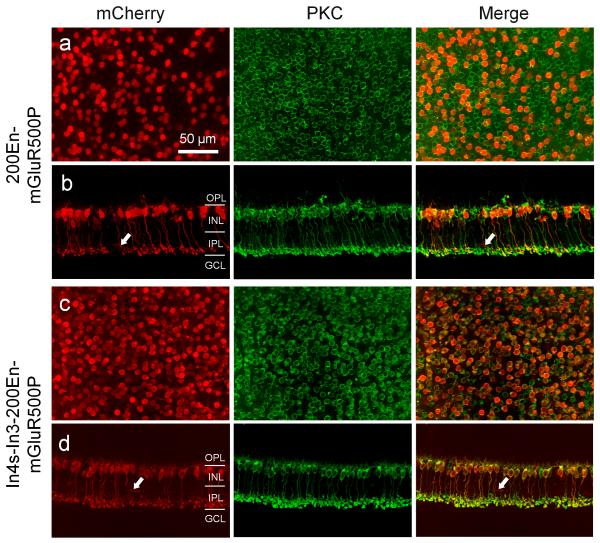
\includegraphics[width=1.0\textwidth]{Lu2016-Fig04.jpg}
\caption{图T2\quad 论文原图（Lu et al., 2016, Fig.~4）：mCherry（红）与视杆双极细胞标记 PKC 的共标结果。}
\end{figure}

\begin{figure}[H]
\centering
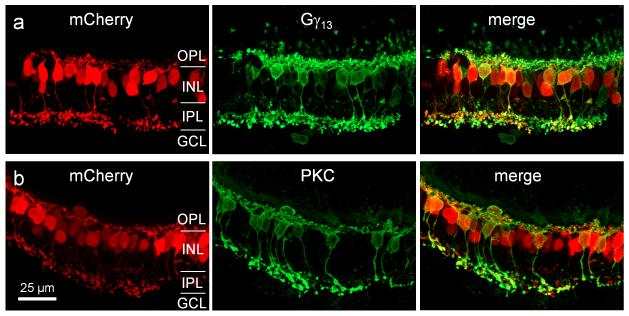
\includegraphics[width=1.0\textwidth]{Lu2016-Fig08.jpg}
\caption{图T3\quad 论文原图（Lu et al., 2016, Fig.~8）：灵长类视网膜（距中央凹 6--8 mm 区域）中 mCherry 与细胞标记的双标结果。}
\end{figure}

\subsection*{设问（共 10 分）}

\begin{enumerate}[leftmargin=2.1em,itemsep=5pt]
\item \tg{单选} \pt{2} 据图T2，mCherry 的荧光信号与 PKC 的荧光信号在\textbf{同一批细胞}中重叠，说明目的基因主要表达在（\quad）\\
\choice{A. 感光细胞 \quad B. 视杆双极细胞 \quad C. 神经节细胞 \quad D. 水平细胞}

\item \tg{多选} \pt{2} 若把 ChR2 基因导入\textbf{感光细胞}，则（\quad）\\
\choice{A. 对 RP 患者没有意义，因为这些细胞已经大量死亡\\
B. 仍能把光信号经双极细胞上传，从而恢复患者视觉\\
C. 该做法不能解决 RP 患者的失明问题\\
D. 只有在感光细胞仍然存活时，该做法才可能有效}

\item \tg{编号选填} \pt{2} 研究者希望目的基因"只在双极细胞中表达、且表达量足够高"。为此应优先考虑改造（\quad）（可填多个编号）\\
\choice{① 病毒衣壳蛋白 \quad ② 目的基因的编码序列 \quad ③ 与目的基因连接的启动子与增强子 \quad ④ 荧光标签蛋白}

\item \tg{编号排序} \pt{2} 用编号和箭头表示\textbf{正常}视网膜内光信号的传递顺序：\\
\choice{① 双极细胞 \quad ② 感光细胞 \quad ③ 神经节细胞 \quad 答：\tian{4.2cm}}

\item \tg{填空} \pt{2} 研究者在灵长类视网膜上重复实验，其主要目的是：\tian{0.5\textwidth}
\end{enumerate}

\ans
\begin{enumerate}[leftmargin=2.1em,itemsep=3pt]
\item \textbf{B}。mCherry 与 PKC（视杆双极细胞的特异性标记）\textbf{共定位}，说明目的基因主要表达在视杆双极细胞中；若答"在视网膜中表达"不得分，必须体现共定位判断。
\item \textbf{ACD}。B 错：RP 患者感光细胞已大量死亡，把光敏蛋白放在其中无法产生并传递信号；D 对：该思路仅在感光细胞仍存活时才有意义。
\item \textbf{①③}。③决定"在哪种细胞表达、表达多少"（特异性与表达量），①（衣壳改造）决定载体进入目标细胞的\textbf{转导效率}；②决定"表达出什么蛋白"，④只是检测标记，二者都不是提高特异性与效率的直接手段。
\item \textbf{②→①→③}。
\item 灵长类的眼球与视网膜结构\textbf{更接近人}，可检验该策略在更接近人的动物中是否可行、是否安全，为临床转化提供依据（答出"更接近人／为临床转化提供依据"即可）。
\end{enumerate}

\clearpage
\section{题三 · 实验设计型（科学探究）}
\addcontentsline{toc}{section}{题三 · 实验设计型（科学探究）}

\subsection*{材料}

为比较不同 ChR2 变体恢复视功能的效果，研究者把野生型 ChR2（wt）与三种光敏性更高的突变体（L132C、L132C/T159C、L132C/T159S）分别用 rAAV2 载体导入\textbf{三敲除失明小鼠}的视网膜内层神经元（另设注射溶剂的对照组），在相同条件下饲养后测定两项指标：\textbf{视动反应（OMR）}——小鼠头部随视野中移动条纹产生的跟随运动（装置见图T4）；\textbf{瞳孔对光收缩}——光照引起瞳孔缩小的程度（结果见图T5）。图T6 是另一组实验：用阿托品阻断瞳孔收缩后，观察其对 OMR 的影响。

\begin{figure}[H]
\centering
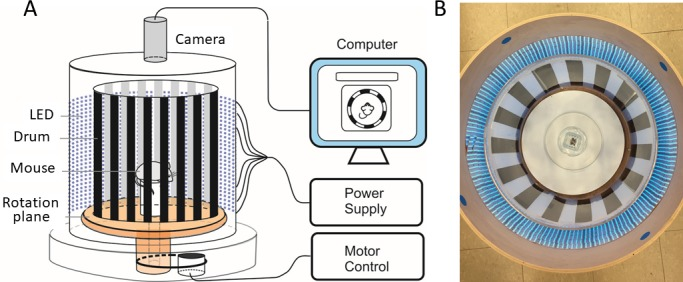
\includegraphics[width=0.86\textwidth]{Lu2018-Fig01.jpg}
\caption{图T4\quad 论文原图（Lu et al., \textit{IOVS}, 2018, Fig.~1）：自制视动反应（OMR）装置。}
\end{figure}

\begin{figure}[H]
\centering
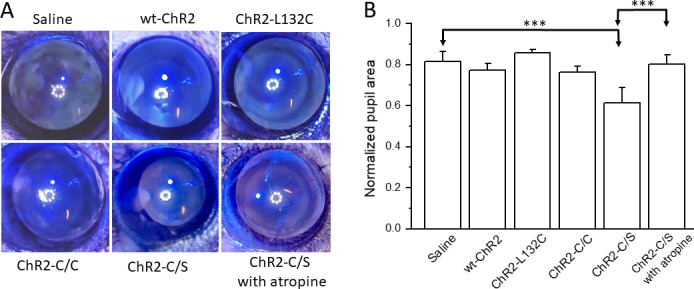
\includegraphics[width=1.0\textwidth]{Lu2018-Fig03.jpg}
\caption{图T5\quad 论文原图（Lu et al., 2018, Fig.~3）：各组小鼠瞳孔对光收缩的比较。}
\end{figure}

\begin{figure}[H]
\centering
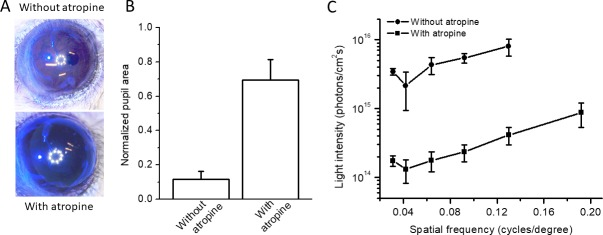
\includegraphics[width=0.95\textwidth]{Lu2018-Fig05.jpg}
\caption{图T6\quad 论文原图（Lu et al., 2018, Fig.~5）：瞳孔收缩对 ChR2 介导光敏性的影响（阿托品阻断）。}
\end{figure}

\subsection*{设问（共 12 分）}

\begin{enumerate}[leftmargin=2.1em,itemsep=5pt]
\item \tg{单选} \pt{2} 本实验的\textbf{自变量}是（\quad）\\
\choice{A. 小鼠是否失明 \quad B. 导入的 ChR2 类型（含溶剂对照组）\\
C. 光刺激的强度与波长 \quad D. 是否出现 OMR}

\item \tg{多选} \pt{2} 为使结论可靠，下列应当\textbf{在各组保持相同（或适宜）}的有（\quad）\\
\choice{A. 小鼠的遗传背景与生理状态 \quad B. 注射的载体体积与浓度\\
C. 注射后至测定的饲养时间 \quad D. 光刺激的波长、强度与时长}

\item \tg{编号排序} \pt{2} 用编号和箭头表示该实验的主要流程：\\
\choice{① 随机分组 \quad ② 注射相应载体或溶剂 \quad ③ 饲养至基因充分表达\\
④ 给予相同光刺激并测定 OMR 与瞳孔直径 \quad ⑤ 比较各组差异 \quad 答：\tian{6.2cm}}

\item \tg{简答} \pt{3} 本实验为什么\textbf{同时}使用"视动反应"与"瞳孔对光收缩"两项指标，而不是只测一项？

\item \tg{简答·实验设计} \pt{3} 有同学指出：瞳孔收缩本身会改变进入眼内的光量，可能干扰 OMR 的测定。请设计一个实验来排除这一干扰（写出处理思路与判断依据）。
\end{enumerate}

\ans
\begin{enumerate}[leftmargin=2.1em,itemsep=3pt]
\item \textbf{B}。各组唯一的主动差别是"注射了哪一种 ChR2 变体"，故自变量是导入的 ChR2 类型（含溶剂对照）；光刺激条件是被控制的无关变量，是否出现 OMR 是因变量。
\item \textbf{ABCD}。四者均须相同或适宜，才能保证组间差异来自自变量。
\item \textbf{①→②→③→④→⑤}。
\item 两项指标反映\textbf{不同通路、不同层次}的视功能，且二者被引出的难易不同：\textbf{瞳孔对光收缩}走较短的\textbf{脑干反射通路}（视网膜→视神经→中脑顶盖前区→动眼神经→瞳孔括约肌）；\textbf{OMR} 则需要中枢对\textbf{移动视觉图像}进行分辨与整合，更接近"看得见东西"（2 分）。同时测定可使两项结果\textbf{互相印证}；并且正因为二者对光敏性的要求不同（本实验中 OMR 在各组均已恢复，而瞳孔对光收缩只在光敏性最高的变体出现），两指标并用反而能\textbf{区分不同变体的效能高低}，比只测一项更有分辨力（1 分）。
\item \textbf{思路}：在相同光照条件下，分别在\textbf{用阿托品（散瞳药物）使瞳孔不能收缩}与\textbf{不作该处理}两种情况下，测定同一批 L132C/T159S 小鼠的 OMR 阈值光强或反应强度，比较两者差异（2 分）。\\
\textbf{判断依据}：若两种情况下 OMR 阈值\textbf{无显著差异}，说明瞳孔收缩对 OMR 测定没有实质影响，原有结论成立；若散瞳后 OMR 明显变差（阈值升高），说明瞳孔收缩确实通过\textbf{增加进光量}参与了 OMR 的产生，原有结论需修正（1 分）。
\emph{评分要点：能写出"阻断瞳孔收缩后重复测定并比较"即得 2 分；提到"同一批动物自身对照"或"人为遮光对照"可满分。}
\end{enumerate}

\clearpage
\section{题四 · 跨学科定量分析型}
\addcontentsline{toc}{section}{题四 · 跨学科定量分析型}

\subsection*{材料}

OMR 的测定需要小鼠能分辨视野中移动的条纹。条纹越\textbf{密集}（空间频率越高），分辨越困难，所需的最低光强也越高。研究者测定了三种变体小鼠在不同空间频率下引起 OMR 的\ \textbf{阈值光强}（图T7）。题三的结果表明：各变体组的 OMR 均能恢复，但只有光敏性最高的 ChR2-L132C/T159S 组出现显著的瞳孔对光收缩。

\begin{figure}[H]
\centering
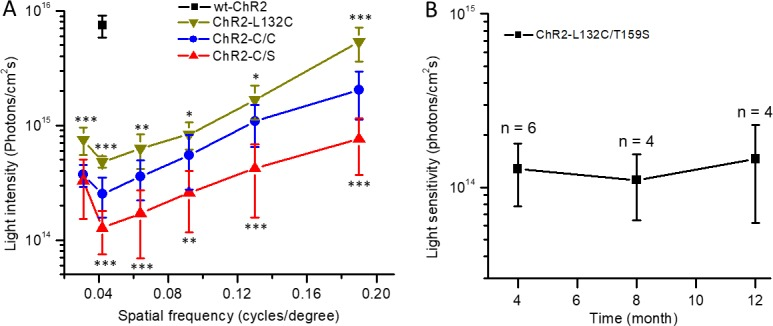
\includegraphics[width=1.0\textwidth]{Lu2018-Fig04.jpg}
\caption{图T7\quad 论文原图（Lu et al., 2018, Fig.~4）：不同 ChR2 变体小鼠的 OMR 阈值光强与空间频率的关系（A 为阈值光强—空间频率曲线）。}
\end{figure}

\subsection*{设问（共 10 分）}

\begin{enumerate}[leftmargin=2.1em,itemsep=5pt]
\item \tg{单选} \pt{2} 据图T7，随空间频率（条纹密集程度）升高，引起 OMR 所需的最低光强总体（\quad）\\
\choice{A. 逐渐升高 \quad B. 逐渐降低 \quad C. 保持不变 \quad D. 先升高后降低}

\item \tg{多选} \pt{2} 关于"阈值光强"，下列说法正确的有（\quad）\\
\choice{A. 同一空间频率下，阈值光强越低，说明该组细胞对光越敏感\\
B. 可用"逐级改变光强、取刚好出现 OMR 的最小光强"来确定阈值\\
C. 阈值光强与细胞的光敏性无关\\
D. 阈值光强可作为评价光遗传学工具效能的一项指标}

\item \tg{编号选填} \pt{2} 结合题三结果推测：在相同空间频率下，阈值光强最低的曲线应来自（\quad）\\
\choice{① ChR2-L132C \quad ② ChR2-L132C/T159C \quad ③ ChR2-L132C/T159S}

\item \tg{填空} \pt{2} 写出"阈值光强"的含义，并说明实验中如何用数据确定它：\tian{0.5\textwidth}

\item \tg{简答} \pt{2} 从工程（应用）角度说明：为什么"提高弱光下的光敏性"对光遗传学疗法的临床应用特别重要？
\end{enumerate}

\ans
\begin{enumerate}[leftmargin=2.1em,itemsep=3pt]
\item \textbf{A}。条纹越密越难分辨，需要更强的光才能引出 OMR，故阈值光强总体升高（曲线在较高空间频率处增速变缓，趋于饱和）。
\item \textbf{ABD}。C 错：阈值光强越低表示在越弱的光下即可产生反应，即光敏性越高，二者直接相关。
\item \textbf{③}。题三已表明 L132C/T159S 的光敏性最高（唯一能引起显著瞳孔收缩），故在相同空间频率下它所需的阈值光强最低。
\item \textbf{含义}：在给定空间频率下，能引起\textbf{可观测 OMR 的最低光强}（1 分）。\\
\textbf{确定方法}：在同一空间频率下由低到高\textbf{逐级改变光强}，记录是否出现 OMR，取"刚好出现稳定 OMR"的最小光强作为该频率下的阈值（1 分）。
\item ① 进入眼内的光量本身有限（瞳孔、屈光介质与眼球大小的限制），环境光多为弱光；② 患者需要在\textbf{日常光环境}下获得有用的视觉信息，若必须依靠强光才有反应，实际使用价值很低；③ 提高光敏性还可\textbf{降低所需刺激光强}，减少强光对视网膜的潜在损伤（答出两点即可，每点 1 分）。
\end{enumerate}

\clearpage
\appendix
\section{附录 A\quad 论文原图清单（22 张）}
\addcontentsline{toc}{section}{附录 A\quad 论文原图清单（22 张）}

\noindent 位于 \texttt{00 - Personal/Resources/Downloads/原图-光遗传学视觉恢复/}。\textbf{加粗}者为本卷已使用。

\begin{longtable}{@{}p{2.6cm}p{11.6cm}@{}}
\toprule
\textbf{文件} & \textbf{图注要点（据 PMC 原图注整理）} \\
\midrule
\endhead
\textbf{Lu2016-Fig01} & mGluR6 基因 25 kb 序列示意（翻译起点上游 10 kb + 内含子序列），白框为非编码候选调控序列——\textbf{题一（3）使用} \\
Lu2016-Fig02 & 视网膜铺片荧光图像（分别聚焦内核层与神经节细胞层）+ 垂直切片 \\
Lu2016-Fig03 & 携带 In4s-In3-200En-mGluR500P 启动子的载体在两种衣壳变体下的铺片图像 \\
\textbf{Lu2016-Fig04} & mCherry 与视杆双极细胞标记 PKC 的共标——\textbf{题二（1）使用} \\
Lu2016-Fig05 & 同上的共标与三重标记结果 \\
Lu2016-Fig06 & 两种衣壳变体下 mCherry 的铺片表达 + 局部放大 \\
Lu2016-Fig07 & mCherry、G$\gamma$13、PKC 三重免疫标记 \\
\textbf{Lu2016-Fig08} & 灵长类视网膜（距中央凹 6--8 mm）的双标结果——\textbf{题二（5）使用} \\
\textbf{Lu2018-Fig01} & 自制 OMR 装置（侧视示意 + 俯视照片）——\textbf{题三使用} \\
Lu2018-Fig02 & 三敲除小鼠视网膜中 ChR2s-GFP 的长期稳定表达 \\
\textbf{Lu2018-Fig03} & 各变体小鼠瞳孔对光收缩的比较——\textbf{题三使用} \\
\textbf{Lu2018-Fig04} & OMR 阈值光强—空间频率关系——\textbf{题四使用} \\
\textbf{Lu2018-Fig05} & 阿托品阻断瞳孔收缩对 OMR 光敏性的影响——\textbf{题三（5）干扰排除的依据} \\
Pan2014-Fig01--09 & 132／159 位点 ChR2 突变体的构建与功能鉴定（HEK 细胞与小鼠视网膜神经节细胞光电流记录）——\textbf{题一（5）的素材} \\
\bottomrule
\end{longtable}

\section{附录 B\quad 重绘图（备选配图）}
\addcontentsline{toc}{section}{附录 B\quad 重绘图（备选配图）}

\begin{figure}[H]
\centering
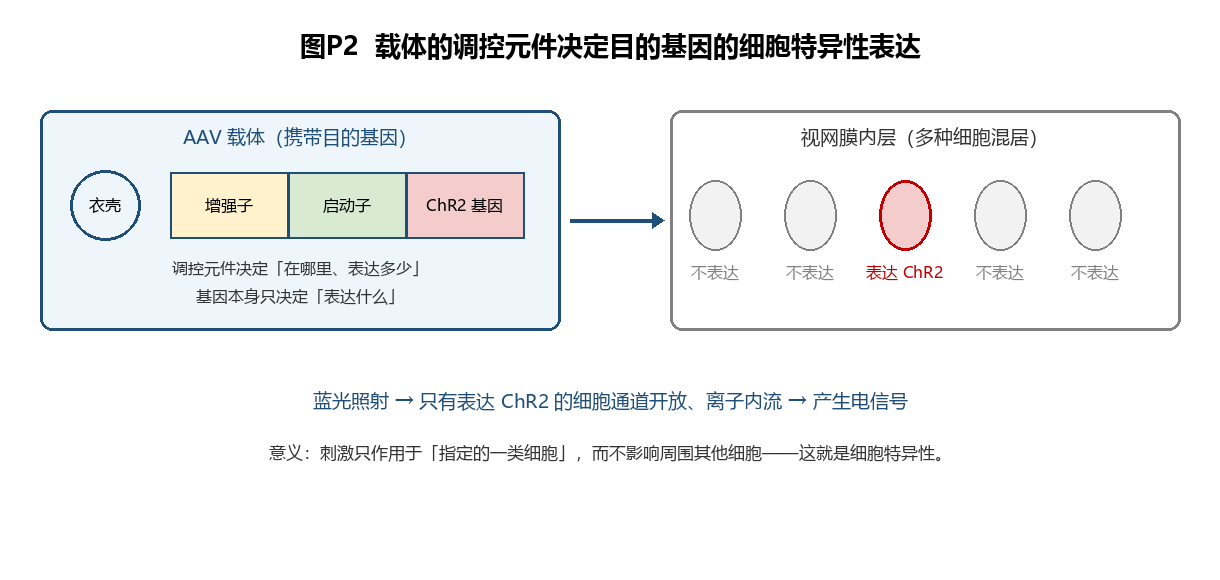
\includegraphics[width=0.9\textwidth]{P2_AAV载体与启动子特异性.png}
\caption{图P2\quad 重绘：载体的调控元件决定目的基因的细胞特异性表达（可替换题一图T1 作入门版）}
\end{figure}

\begin{figure}[H]
\centering
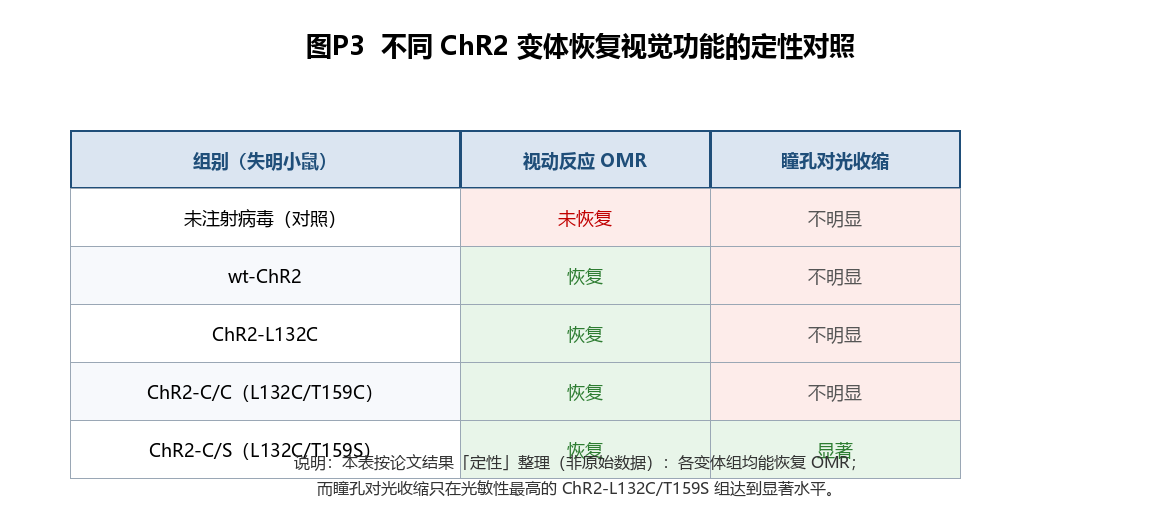
\includegraphics[width=0.8\textwidth]{P3_功能评价定性对照.png}
\caption{图P3\quad 重绘：不同 ChR2 变体恢复视功能的定性对照（非原始数据；可替换题三图T5 作速览版）}
\end{figure}

\section{附录 C\quad 命题质量自检}
\addcontentsline{toc}{section}{附录 C\quad 命题质量自检}

\begin{enumerate}[leftmargin=1.8em,itemsep=2pt]
\item \textbf{题型对齐}：单选 4、多选 4、编号选填 3、编号排序 3、填空 3、简答/设计 4，客观题占比约 64\%，与上海卷"单选、多选、编号选填、填空、简答"的题型结构一致。
\item \textbf{以原图为主}：题干与据图题共使用 7 张论文原图（整栏宽度），重绘图仅 1 张（补足通路示意），其余重绘图移入附录 B 备选。
\item \textbf{情境真实、不超纲}：材料与结果均来自三篇开放获取论文；考点限于物质跨膜运输、基因工程、基因突变、神经调节、反射与实验设计。
\item \textbf{设问递进}：每道大题按 识记 → 图表分析 → 机制推理 → 方案设计 排列，与官方"由浅入深、层层递进"的表述对应。
\item \textbf{答案与评分可操作}：客观题给出唯一答案并标注多选评分规则；简答题逐条列出给分点；开放题注明"言之成理即可"。
\item \textbf{已知局限}：题四（1）（3）的曲线判读以论文原图为准；本命题由程序化方式生成配图与排版，图形细节请在使用前目视复核。
\end{enumerate}

\end{document}
